
\subsection{Proxy-based Contrastive Replay}
\label{sec:PCR}

Our previous work~\cite{Lin_2023_CVPR} analyzes existing studies and proposes to couple two replay manners, achieving complementary advantages. The characteristics of these two replay manners are summarized in Table~\ref{table:characteristics}. For one thing, the anchor-to-proxy pairs of proxy-based replay manner can overcome the disadvantage of contrastive-based loss. For another thing, the contrastive-based loss provides a heuristic way to select anchor-to-proxy pairs for the proxy-based replay manner. Moreover, the anchor-to-sample pairs contain richer fine-grained semantic knowledge than the anchor-to-proxy pairs.

Although there are some coupling solutions, they can not address the forgetting problem at all. For example, the most intuitive way is to add different loss functions as
\begin{equation}
\begin{split}
    \label{eq:coupleloss1}
    L_{couple}^{1}=L_{ER} + L_{SCR}.
\end{split}
\end{equation} 
It is a two-stage strategy for offline learning~\cite{li2022targeted}, which is unsuitable for OCL due to timeliness requirements. Another way is to add anchor-to-sample pairs to cross-entropy loss as
\begin{equation}
\begin{split}
    \label{eq:coupleloss2}
    &
    L_{couple}^{2}=E_{(\bm{x},y)\sim{\mathcal{B}\cup\mathcal{B}_\mathcal{M}}}\\
    &
    [-log(\frac{exp(o_y)}{\sum_{c\in{\mathcal{C}_{1:t}}}exp(o_c)+\sum_{j\in{\mathcal{J}}}exp(\langle \bm{z},\bm{z}_j\rangle/\tau)})].
\end{split}
\end{equation} 
in the work~\cite{yao2022pcl}. Both of them cannot take advantage of each replay manner to address the forgetting issue of OCL. Since they ignore that the key is to select anchor-to-proxy pairs in a contrastive way and train by the selective pairs. 

Therefore, the proxy-based contrastive replay (PCR) framework is proposed by replacing the samples of anchor-to-sample pairs with proxies in the contrastive-based loss. Specifically, the model is trained by learning samples of new classes and replaying samples of old classes in the training procedure. For each step, given current samples $\mathcal{B}$, it randomly retrieves previous samples $\mathcal{B}_\mathcal{M}$ from the memory buffer. Besides, these samples are spliced together for the batch of training. Then, the model is optimized by  
\begin{equation}
    \label{eq:pcrloss}
\begin{split}
    L_{PCR}=E_{(\bm{x},y)\sim{\mathcal{B}\cup\mathcal{B}_\mathcal{M}}}[-log(\frac{exp(o_y)}{\sum_{c\in\mathcal{C}_{1:t}}k_c exp(o_c)})].
\end{split}
\end{equation}
where $k_c$ is the number of samples belonging to class $c$ in the training batch. Different from existing studies, its way of computing categorical probability is changed for each mini-batch. Finally, it updates the memory buffer by reservoir sampling strategy, which can ensure that the probability of each sample being extracted is equal. Conveniently, the memory buffer has a fixed size, no matter how large the sample amount is.

The inference procedure is different from the training procedure. Each testing sample $\bm{x}_k$ obtains its class probability distribution by Equation (\ref{eq:probability}). And PCR performs the inference prediction to $\bm{x}_k$ with highest probability as
\begin{equation}
 	\begin{split}
	 	y_k^* = \mathop{\arg\max}_{c}p_c,y\in C_{1:t}.
 	\end{split}
\end{equation}

% \subsection{Other Classifier}

% If there are sufficient computing resources, The inference procedure (line 11-15) of PCR can also use NCM classifier. Before calculating the probability distribution for a testing sample $\bm{x}_k$, we need obtain the classification centers for learned classes by
% \begin{equation}
%  	\begin{split}
% 	 	\bm{\mu}_c=\frac{1}{n_c}\sum_i^n\bm{z}_i\cdot\mathds{1}\{y_i=c\},c\in C_{1:t}
%  	\end{split}
% \end{equation}
% where $n$ is the number of previous samples in $\mathcal{M}$ and $n_c$ is the number of previous samples belong to class $c$ in $\mathcal{M}$. Finally, we perform the inference prediction to $\bm{x}_k$ with nearest distance as
% \begin{equation}
%  	\begin{split}
% 	 	y^* = \mathop{\arg\min}_{c}\Vert\bm{z}-\bm{\mu}_c\Vert,c\in C_{1:t}.
%  	\end{split}
% \end{equation}

% \subsection{Full Proxy-based Contrastive Replay}


\section{Analysis for Proxy-based Contrastive Replay}

\subsection{Gradient Analysis}
As stated in the previous work~\cite{Lin_2023_CVPR}, gradient analysis is of great help in exploring forgetting problems and existing work. Specifically, the gradient of the softmax classifier for $\bm{x}$ is
\begin{equation}
    \label{eq:gradient_h}
    \frac{\partial L}{\partial <\bm{z},\bm{w}_c>}=\left\{
    \begin{aligned}
        (p_y-1)/\tau&,&c= y \\
        (p_c)/\tau&,&c\neq y
    \end{aligned}
    \right..
\end{equation}
Training $\bm{x}$ belongs to class $y$ provides the positive gradient $-\eta(p_y-1)/\tau$ for the proxy of class $y$ as $<\bm{z},\bm{w}_y>=<\bm{z},\bm{w}_y>-\eta(p_y-1)/\tau$, and propagates the negative gradient $-\eta(p_c)/\tau$ to the other proxies as $<\bm{z},\bm{w}_c>=<\bm{z},\bm{w}_c>-\eta(p_c)/\tau$, where the learning rate $\eta$ is positive. If training as Equation (\ref{eq:oclloss}), the proxies of new classes receive more positive gradients and the others obtain more negative gradients. It causes the proxies of new classes to be close to the samples of new classes, while the proxies of old classes are far away from the samples of new classes. Hence, it is easy to classify most samples into new classes, causing the forgetting problem. If replaying as Equation (\ref{eq:erloss}), the proxies of old classes can obtain more positive gradient, and the proxies of new classes receive more negative gradient. Although the forgetting can be mitigated, its effect is still limited by the imbalanced samples.  

To explore the reliability of PCR, we analyze its gradient propagation process. Similar to Equation (\ref{eq:gradient_h}), the gradient of the classifier for a sample $\bm{x}$ in PCR is stated as Theorem~\ref{thm1}.
\newtheorem{theorem}{\bf Theorem}
\begin{theorem}\label{thm1}
	In PCR, the gradient for all proxies is 
 \begin{equation}
    \label{eq:gradient_pcr}
    \frac{\partial L_{PCR}}{\partial <\bm{z},\bm{w}_c>}=\left\{
    \begin{aligned}
        (k_yp^*_y-1)/\tau&,&c= y \\
        (k_cp^*_c)/\tau&,&c\neq y
    \end{aligned}
    \right.,
\end{equation}
where 
\begin{equation}
\begin{split}
    p^*_y=\frac{exp(o_y)}{\sum_{c\in\mathcal{C}_{1:t}}k_j exp(o_c)}.
\end{split}
\end{equation}
\end{theorem} 
When replaying, the number of classes is relatively small and the number of samples is relatively large for new classes; the number of classes is relatively large and the number of samples is relatively small for old classes. It means that in a training batch, the number of samples for new classes tends to be multiple, while the one for old classes tends to be small, or even non-existent. Based on this situation, Equation~(\ref{eq:gradient_pcr}) demonstrates two advantages of PCR for anti-forgetting. 

For one thing, the gradient only influences the classes whose associated samples exist in the same training batch. For example, when learning a current sample $\bm{x}$ belongs to class $y$, the gradient for the proxy of class $c (c\neq y)$ is $-\eta(k_cp^*_c)/\tau$ if there are $k_c$ samples belonging to class $c$ in the same batch. Otherwise, if $k_c=0$, the proxy of class $c$ does not participate in the gradient propagation. Due to the lower probability of old classes appearing in the training batch, the proxies of old classes will receive fewer negative gradients from the new classes. Thus, the model will keep more historical knowledge. 

Another thing is that the gradient can be affected by the number of samples in a training batch. Conveniently, we define
\begin{equation}
\begin{split}
    {sum}_y=\sum_{c\in\mathcal{C}_{1:t},c\neq y}k_cexp(o_c).
\end{split}
\end{equation}
With this representation, the Equation~(\ref{eq:gradient_pcr}) can be changed to 
 \begin{equation}\small
    \label{eq:gradient_pcr_other}
    \frac{\partial L_{PCR}}{\partial <\bm{z},\bm{w}_c>}=\left\{
    \begin{aligned}
        (\frac{k_yexp(o_y)}{{sum}_y+k_yexp(o_y)}-1)/\tau&,&c= y \\
        \frac{k_cexp(o_c)}{{sum}_y+k_yexp(o_y)}/\tau&,&c\neq y
    \end{aligned}
    \right..
\end{equation}
We take the training batch including $k_i (k_i\geq1)$ samples of new class $i$ and $k_j (k_j=1)$ samples of other old classes $j$ as an example. Training new class $i$ propagates the gradient as  
\begin{equation}\small
    \frac{\partial L_{PCR}}{\partial <\bm{z},\bm{w}_c>}=\left\{
    \begin{aligned}
        -\frac{{sum}_i}{{sum}_i+k_iexp(o_i)}/\tau&,&c= i \\
        \frac{exp(o_c)}{{sum}_i+k_iexp(o_i)}/\tau&,&c= j
    \end{aligned}
    \right..
\end{equation}
At this moment, the larger the $k_i$ is, the smaller the $\frac{1}{{sum}_i+k_iexp(o_i)}$ is, and the smaller the gradient value is. It means that the larger $k_i$ can reduce the positive gradient for the proxy of new class $i$ and the negative gradient for the proxy of old classes $j$. Similarly, training any old class $j$ propagates the gradient as
\begin{equation}\small
    \frac{\partial L_{PCR}}{\partial <\bm{z},\bm{w}_c>}=\left\{
    \begin{aligned}
        (\frac{exp(o_c)}{{sum}_i+k_iexp(o_i)}-1)/\tau&,&c= j \\
        (1-\frac{{sum}_i}{{sum}_i+k_iexp(o_i)})/\tau&,&c=i
    \end{aligned}
    \right..
\end{equation}
In this situation, the larger the $k_i$ is, the smaller the $\frac{1}{{sum}_i+k_iexp(o_i)}$ is, and the larger the gradient value is. With larger $k_i$, both the positive gradient for old class $j$ and the negative gradient for the new class $i$ can be increased. Therefore, PCR helps old classes acquire some advantages in the propagation of gradient, and the gradient propagation efficiency of these selected proxies will be greatly improved.

\subsection{Limitation Analysis}
Based on the gradient analysis, we can find that PCR can help the model alleviate the phenomenon of catastrophic forgetting. It selects partial proxies instead of all to learn current samples and replay previous samples. In such a learning way, the old classes whose associated samples are not selected can avoid the bias caused by unbalanced gradient competition.

However, PCR remains suboptimal due to several unaddressed limitations. Firstly, PCR exclusively considers the relationships of anchor-to-proxy but ignores the relations of anchor-to-sample, leading to the model losing some important semantic information. Anchor-to-sample pairs play a crucial role in enhancing the model's feature extraction capability in large training batches, a vital aspect of PCR. Secondly, the simplistic setting of the temperature coefficient $\tau$ in PCR lacks sophistication. As the temperature coefficient influences PCR's gradient propagation process, employing a static constant is insufficient to ensure the model's generalization ability. Thirdly, those old classes that have been selected to learn together with new classes still face the issue of bias in the training process. It means that the model's anti-forgetting ability still can be further improved. In a word, PCR can be improved into a more holistic and effective approach.

\section{Holistic Proxy-based Contrastive Replay}
\label{sec:PCR+}
In this work, we develop a more comprehensive and effective method called holistic proxy-based contrastive replay (HPCR). HPCR consists of a contrastive component, a temperature component, and a distillation component, resolving the limitations of PCR in sequence. 

\subsection{Contrastive Component}
 The contrastive component conditionally incorporates the anchor-to-sample pairs to PCR and improves the model's ability of feature extraction. The anchor-to-sample pairs contain richer fine-grained semantic information compared to anchor-to-proxy pairs. Although extracting the relations of anchor-to-sample is easily limited by the number of samples in a training batch, it can still play a crucial role when the batch size is sufficient. Hence, the contrastive component of HPCR is denoted as 

\begin{equation}\small
    \label{eq:pcr+}
\begin{split}
    &
    L_{PCR_{C}}=E_{(\bm{x},y)\sim{\mathcal{B}\cup\mathcal{B}_\mathcal{M}}}[\frac{-1}{|\mathcal{P}|}\sum_{p\in\mathcal{P}}
    \\
    &
    log(\frac{exp(o_y)+s(N)\cdot exp(\langle \bm{z},\bm{z}_p\rangle/\tau)}{\sum_{c\in\mathcal{C}_{1:t}}k_c exp(o_c)+\sum_{j\in\mathcal{J}} s(N)\cdot exp(\langle\bm{z},\bm{z}_j\rangle/\tau)})].
\end{split}
\end{equation}
Here, $s(N)$ is a self-defined step function used to control the importance of anchor-to-sample pairs, and it is defined as
\begin{equation}
\label{eq:step_function}
    s(N)=\left\{
    \begin{aligned}
        0,\quad&N < N_{min}\\
        1,\quad&N \geq N_{min}
    \end{aligned}
    \right..
\end{equation}
$N$ is the number of samples in the current training batch, and $N_{min}$ is a hyper-parameter used to determine whether to use anchor-to-sample pairs. When the size of the training batch is small, the correlation between samples is prone to noise affecting the performance of the model. Therefore, their importance should be set to 0. At this point, $\rm PCR_C$ degenerates into PCR; otherwise, the importance of these samples should be set to 1 to improve the model's feature extraction ability. Compared to the PCR, $\rm PCR_C$ can not only mine the relations of anchor-to-proxy, but also explore the relations of anchor-to-sample. It increases inter-class distance as well as decreases intra-class distance.
\begin{figure*}[t]
\centering
    \begin{minipage}[t]{0.44\linewidth}
        \centering
        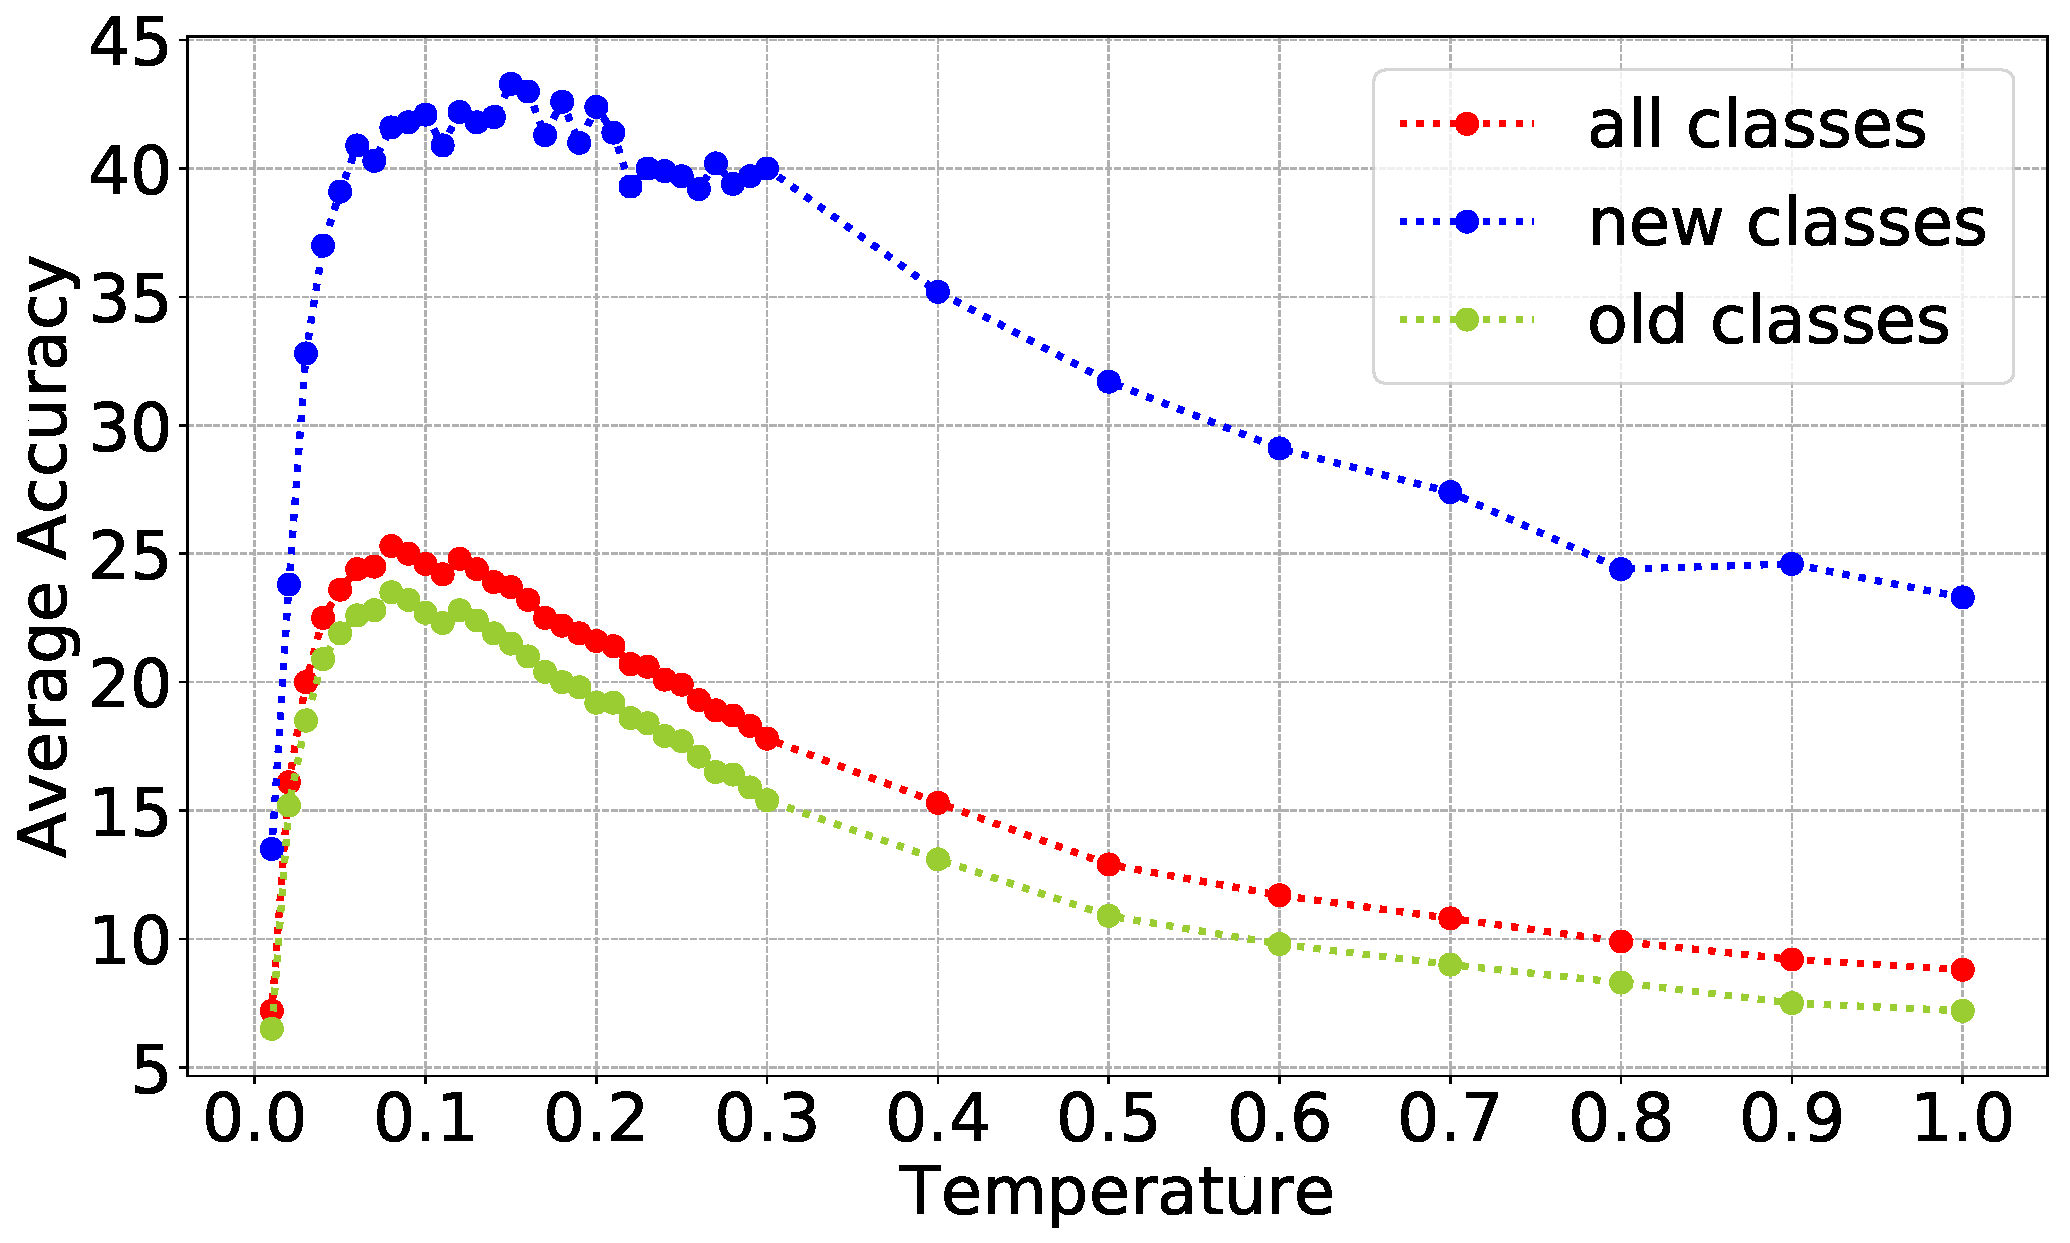
\includegraphics[scale=0.22]{sections/Figures/pcr_cifar100_tau.pdf}
        {(a) The performance on different classes}
    \end{minipage}
    \begin{minipage}[t]{0.44\linewidth}
        \centering
        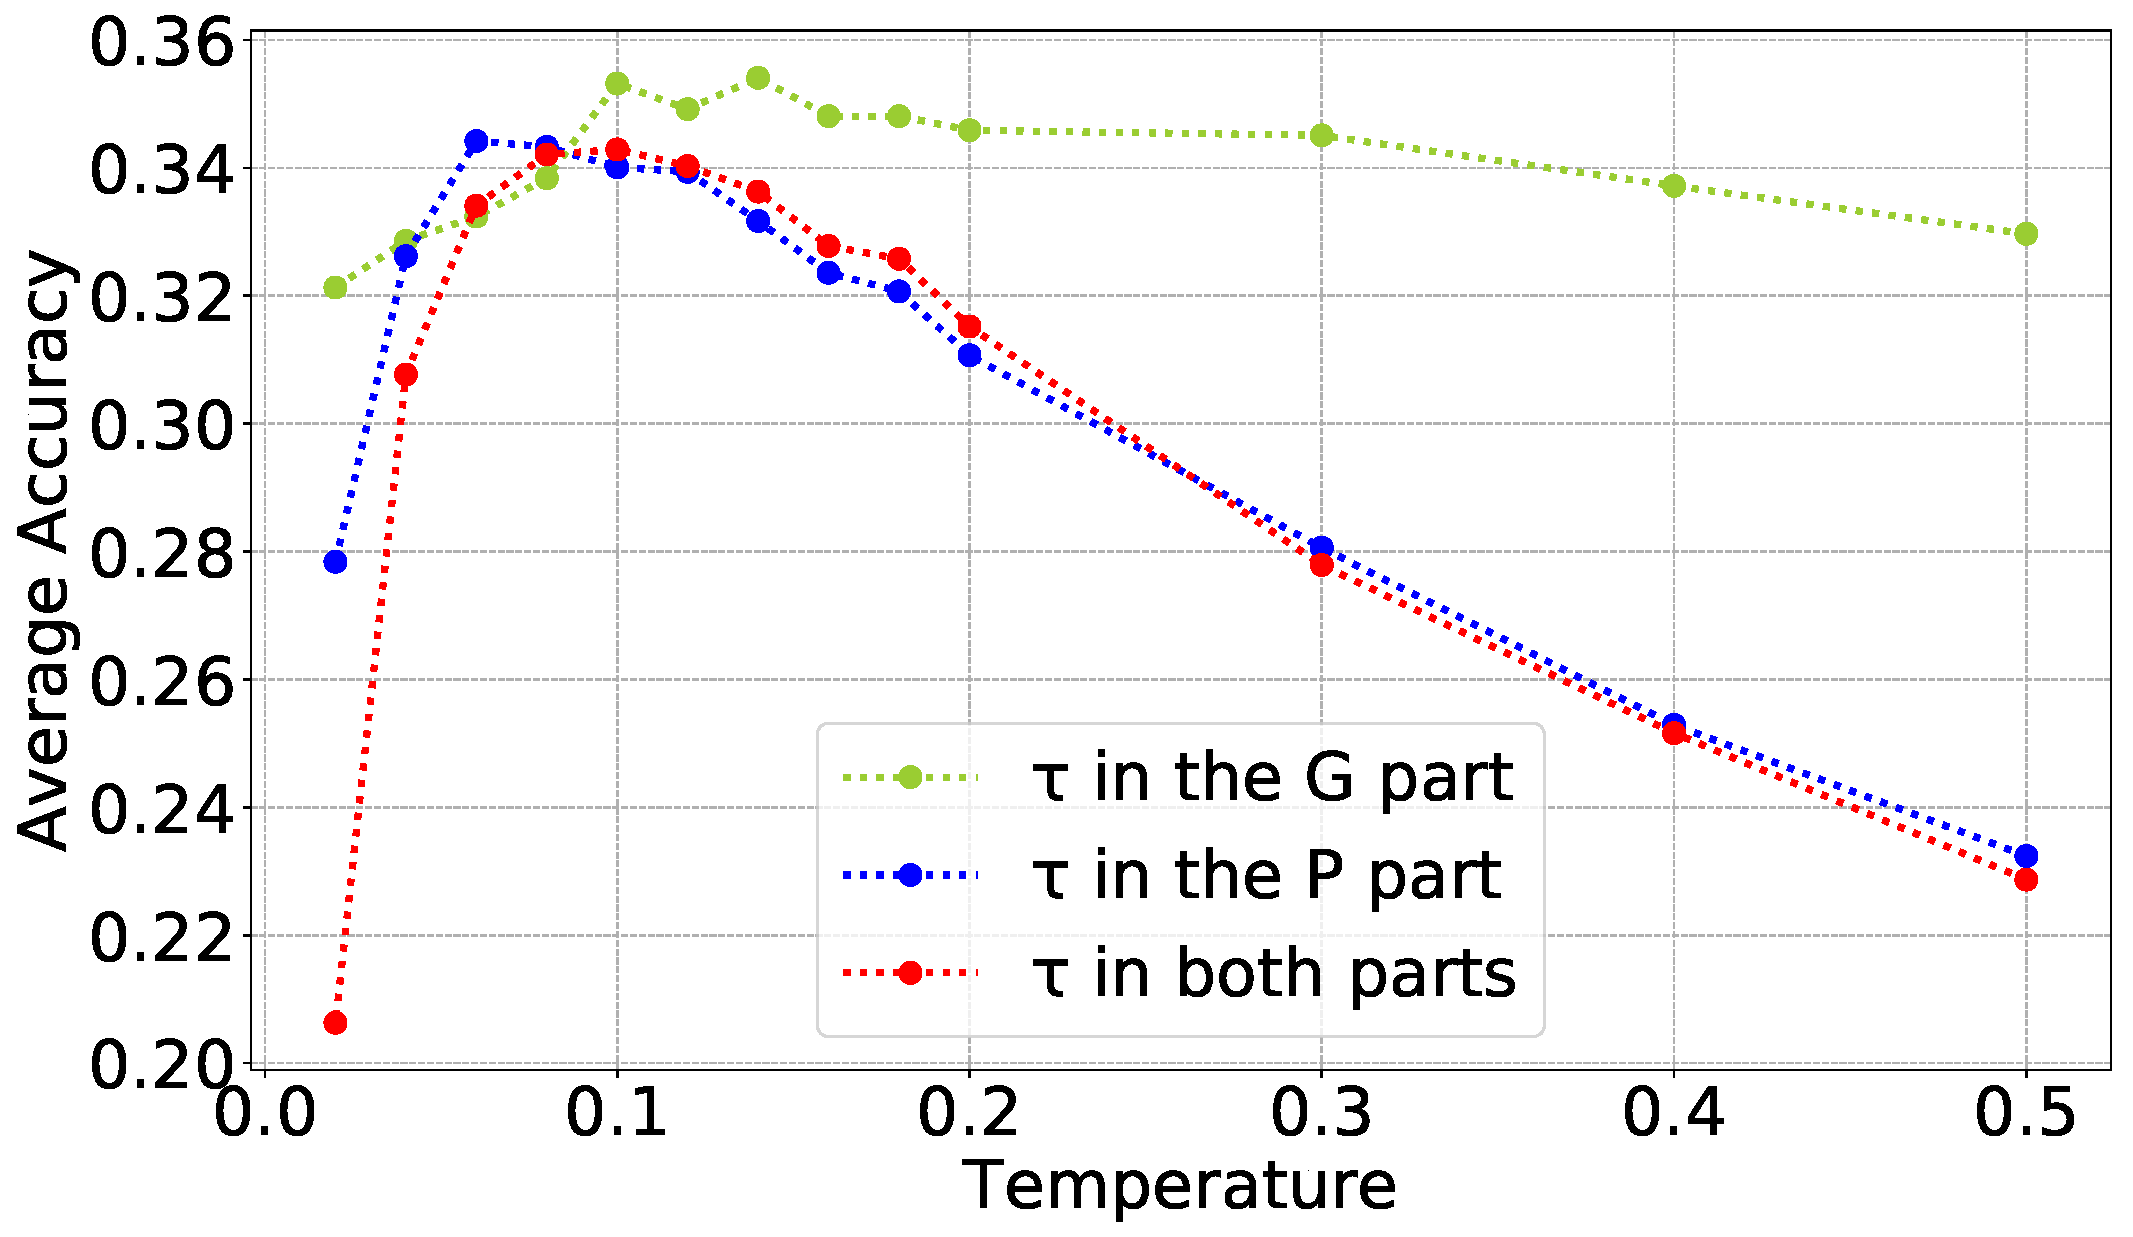
\includegraphics[scale=0.22]{sections/Figures/pcr_cifar100_tau_both.pdf}
        {(b) The performance on different parts}
    \end{minipage}
\centering
\vspace{-1ex}
\caption{The performance of PCR on Split CIFAR100 (buffer size=1000) with different value of $\tau$. }
\label{fig:tau}
\vspace{-2ex}
\end{figure*}



\subsection{Temperature Component}

\subsubsection{The Analysis of Temperature Coefficient}
In Equation (\ref{eq:gradient_pcr}), the gradient propagation is influenced by $\tau$, which is called the temperature coefficient. In a proxy-based classifier, the norm of vectors has been proved to be unfriendly to continual learning and thus abandoned~\cite{hou2019learning}. However, the retained similarity of vectors $\langle\bm{z},\bm{w}\rangle$ has a value range of $[-1,1]$, which brings certain difficulties to the optimization of the model. Hence, $\tau$ in $p^*_c$ is used to control the strength of $\langle\bm{z},\bm{w}\rangle$, which is vital to find the optimal solution. 

Inspired by~\cite{wang2021understanding}, we define a relative penalty $r(\langle\bm{z},\bm{w}_c\rangle)$ on negative proxy $\bm{w}_c(c\neq y)$ for the sample $(\bm{x},y)$ by
\begin{equation}
    \begin{split}
    r(\langle\bm{z},\bm{w}_c\rangle)=\frac{|\frac{\partial L}{\partial <\bm{z},\bm{w}_c>}|}{|\frac{\partial L}{\partial <\bm{z},\bm{w}_y>}|}=\frac{k_cexp(o_c)}{\sum_{j\neq y}k_jexp(o_j)}, c\neq y.
    \end{split}
\end{equation}
It can reflect the strength of penalties on all negative samples. As $\tau$ increases, the distribution of $r(\langle\bm{z},\bm{w}_c\rangle)$ is relatively uniform, and the model tends to treat all negative proxies with the same strength. On the contrary, the model focuses on the negative proxies with higher similarities when $\tau$ decreases.

Furthermore, within a reasonable interval, smaller $\tau$ is more suitable for replaying old classes, while larger $\tau$ is more effective for learning new classes in OCL. Generally, the number of samples in old classes is small, while the number of samples in new classes is large in OCL. It leads to the samples of old classes being more likely to become negative samples with shorter distances, while the samples of new classes tend to become negative samples with larger distances. As a result, large $\tau$ will prompt the model to pay attention to the samples of new classes with larger distances, making it easy to ignore samples from old classes. In contrast, small $\tau$ will urge the model to focus on the samples of old classes with shorter distances, resulting in the information loss from new classes.

Finally, as seen in Equation (\ref{eq:gradient_pcr}), $\tau$ affects the process in two parts. First, it directly changes the value of the gradient by ${1}/{\tau}$ (denoted as G part). Second, it smooths the probability distribution $p^*_c$ of samples to implicitly adjust the gradient (denoted as P part). Moreover, the P part has a more complex impact than the G part due to its stronger non-linearity. 

\subsubsection{The Influence of Temperature Coefficient}
The performance of PCR would be highly sensitive to $\tau$. To validate this viewpoint, we conduct experiments for PCR with different values of $\tau$, and the results are shown in Figure~\ref{fig:tau}.
In addition to the final accuracy rate of all classes, we also report the ones of new and old classes separately. In Figure~\ref{fig:tau}(a), we can make the following observations: 1) The performances of all, old, and new classes are sensitive to $\tau$. For example, when $\tau$ changes from 0.01 to 0.2, the performance of PCR in all aspects would first increase and then decrease. 2) The sensitivity of old and new classes w.r.t. $\tau$ is different, and their best $\tau$ are different. The performance on new classes reaches the best result when $\tau\in[0.1,0.2]$ while the performance on old classes reaches the best result when $\tau\in[0.0,0.1]$. 

At the same time, we also demonstrate the performance when different $\tau$ are taken in different parts. In Figure~\ref{fig:tau}(b), the lines of green, blue, and red denote the performance when $\tau$ changes in the G part, the P part, and both parts. For the G part, we keep $\tau=0.09$ for $p^*_c$ and only change the value of $\tau$ for ${1}/{\tau}$. On the contrary, $\tau$ is set as 0.09 for ${1}/{\tau}$ and changed from 0.0 to 0.5 in the P part. Comparing the results of the two cases, we find that the performance of the model is more sensitive to changes in $\tau$ in the G part. Meanwhile, the model exhibits greater fluctuations when $\tau$ reaches the optimal value in the P part. Although the performance of the P part appears stable with changes in $\tau$, the accuracy of each class actually changes. Conveniently, we report the best $\tau$ for each class on Split CIFAR10 in the P part when the buffer size is 100. As stated in Table~\ref{table:tau}, to achieve the highest accuracy, the value of $\tau$ for each class is different. In a word, the setting of $\tau$ in the P part is sensitive, and a static value is more suitable for it. While a dynamic value is more suitable for the G part since it allows the model to consider different classes. Therefore, the setting of $\tau$ for these two parts should be decoupled.

\begin{table}[t]
\renewcommand\tabcolsep{4pt}
\centering
\caption{The best $\tau$ for each class on Split CIFAR10 (buffer size=100).}
\vspace{-1ex}
\label{table:tau}
\begin{tabular}{l|llllllllll}
\hline
class & 0    & 1    & 2    & 3    & 4    & 5    & 6    & 7    & 8    & 9    \\ \hline
type  & old  & old  & old  & old  & old  & old  & old  & old  & new  & new  \\
$\tau$     & 0.01 & 0.14 & 0.16 & 0.17 & 0.12 & 0.20 & 0.06 & 0.09 & 0.14& 0.2 \\ \hline
\end{tabular}
\vspace{-4ex}
\end{table}

\subsubsection{Decoupled Temperature Coefficient}
To this end, we set different values of $\tau$ for the P and G parts separately. For one thing, since the performance of the model is more sensitive to the P part, we set it to a static constant value. Meanwhile, we obtain a moderate value to balance the model's attention to new and old classes using the grid search method. For another thing, due to the different optimal $\tau$ for each class, we set a dynamic one for the G part. However, it is highly difficult to find an optimal $\tau$ for each class at any time, since the real-time requirement of OCL is high. In such a situation, the dynamic temperature is set as a robust function independent of the class, and the function is denoted as
\begin{equation}
\label{eq:tau_t}
 	\begin{split}
	 	\tau(s) = (\tau_{max}-\tau_{min})\times(1+cos(2\pi s/S))/2+\tau_{min},
 	\end{split}
\end{equation}
where $s$ is the current step, $S$ is the cycle length, $\tau_{max}$ is the upper bound, and $\tau_{min}$ is the lower bound. With such a periodic dynamic function, the model can select a wide range of different temperature values during the OCL process. It improves the accuracy of each class and thus enhances the overall generalization ability of the model. Therefore, the Equation (\ref{eq:pcr+}) can be improved to
\begin{equation}\small
\label{eq:pcr++}
\begin{split}
&
L_{PCR_{CT}}=E_{(\bm{x},y)\sim{\mathcal{B}\cup\mathcal{B}_\mathcal{M}}}[\frac{-1}{|\mathcal{P}|}\sum_{p\in\mathcal{P}}\frac{\tau}{\tau(s)}
    \\
    &
    log(\frac{exp(o_y)+s(N)\cdot exp(\langle \bm{z},\bm{z}_p\rangle/\tau)}{\sum_{c\in\mathcal{C}_{1:t}}k_c exp(o_c)+\sum_{j\in\mathcal{J}} s(N)\cdot exp(\langle\bm{z},\bm{z}_j\rangle/\tau)})].
\end{split}
\end{equation}
Moreover, its corresponding gradient is transformed into

\begin{equation}
    \label{eq:gradient_pcr++}
    \frac{\partial L_{PCR_{CT}}}{\partial <\bm{z},\bm{w}_c>}=\left\{
    \begin{aligned}
        (k_yp^*_y-1)/\tau(s)&,&c= y \\
        (k_cp^*_c)/\tau(s)&,&c\neq y
    \end{aligned}
    \right..
\end{equation}


\subsection{Distillation Component}
As a method of knowledge distillation~\cite{hinton2015distilling}, DER~\cite{buzzega2020dark} tries to retain the logits output obtained from the model during learning as historical knowledge for sample replaying. This is to improve the diversity of historical knowledge and avoid the problem of knowledge singularity caused by saving old models to store historical knowledge. However, existing DER has to use all proxies to calculate a loss function of distillation. If distilling as DER, the proxies excluded by PCR will continue to participate in gradient propagation. 

To avoid this situation, we propose a novel distillation method called proxy-based contrastive distillation (PCD). Similar to PCR, the categorical probability in PCD only uses the proxies that appear in the training batch. Specifically, when saving a current sample into the memory buffer, we not only save its instance $\bm{x}$ and label $y$, but also store its logits output of classifier $\bm{o}^*$. If the sample is selected as a previous sample to replay, its $\bm{o}^*$ can be used to keep richer historical knowledge. Hence, we can calculate the PCD loss by minimizing the Euclidean distance between the weighted logits as

\begin{equation}
\label{eq:pcd}
\begin{split}
    L_{PCD}=E_{(\bm{x},y,\bm{o}^*)\sim{\mathcal{B}_\mathcal{M}}}[-\sum_{c}^{\mathcal{C}_{1:t}}k_c(o_c-o^*_c)^2].
\end{split}
\end{equation}

In addition to the distribution distillation of previous samples, relation distillation between samples is also necessary. Since the relation of samples not only reflects intra-class information, but also includes inter-class correlation. Hence, we propose to compute sample-based contrastive distillation (SCD) by $\bm{z}^*$ in a training batch as
\begin{equation}\small
\label{eq:scd}
\begin{split}
    &
    L_{SCD}=E_{(\bm{x},y,\bm{z}^*)\sim{\mathcal{B}_\mathcal{M}}}\\
    &
    [-\sum_{i\in\mathcal{J}}(\frac{exp(\langle\bm{z},\bm{z}_i\rangle/\tau)}{\sum_{j\in\mathcal{J}}exp(\langle\bm{z},\bm{z}_j\rangle/\tau)}log\frac{exp(\langle\bm{z}^*,\bm{z}^*_i\rangle/\tau)}{\sum_{j\in\mathcal{J}}exp(\langle\bm{z}^*,\bm{z}^*_j\rangle/\tau})],
\end{split}
\end{equation}
where $\mathcal{J}$ is the indices set of samples except for anchor $\bm{x}$ in the same batch $\mathcal{B}_\mathcal{M}$. With these two distillation loss functions, the model can transfer more positive gradients to the proxies of old classes and more negative gradients to the proxies of new classes. As a result, the model's ability of anti-forgetting can be improved.



\begin{algorithm}[t]
\caption{Holistic Proxy-based Contrastive Replay}
\label{alg:hpcr}
\textbf{Input}: Dataset $D$, Learning Rate $\lambda$, Scale factor $\tau$\\
\textbf{Output}:Network Parameters $\theta$\\
\textbf{Initialize}:Memory Buffer $\mathcal{M}\leftarrow\{\}$, Network Parameters $\bm{\theta}=\{\bm{\Phi},\bm{W}\}$
\begin{algorithmic}[1]
\FOR{$t\in\{1,2,...,T\}$}
\STATE //$Training\ Procedure$
    \FOR{mini-batch $\mathcal{B}\subset D_t$}
        \FOR{$(\bm{x},y) \in \mathcal{B}$}
            \STATE $\bm{z}=h(\bm{x};\bm{\Phi})$ 
            \STATE $\bm{o}=f(\bm{z};\bm{W})$
            \STATE $(\bm{x},y)\leftarrow(\bm{x},y,\bm{o},\bm{z})$
        \ENDFOR
        \STATE$\mathcal{B}_\mathcal{M}\leftarrow RandomRetrieval(\mathcal{M})$
        \STATE$\mathcal{B}\cup\mathcal{B}_\mathcal{M}\leftarrow Concat([\mathcal{B},\mathcal{B}_\mathcal{M}])$
        \STATE$L_{PCR_{CT}}\leftarrow$Equation~(\ref{eq:pcr++})
        \STATE$L_{PCD}\leftarrow$Equation~(\ref{eq:pcd})
        \STATE$L_{SCD}\leftarrow$Equation~(\ref{eq:scd})
        \STATE$L\leftarrow$Equation~(\ref{eq:hpcr})
        \STATE$\theta\leftarrow\theta+\lambda\nabla_{\theta}L$
        \STATE$\mathcal{M}\leftarrow ReservoirUpdate(\mathcal{M},\mathcal{B})$
    \ENDFOR
\STATE //$Inference\ Procedure$
\STATE $m\leftarrow number\ of\ testing\ samples$

    \FOR{$k\in\{1,2,...,m\}$}
    \STATE $y_k^*\leftarrow \mathop{\arg\max}_{c}p_c,c\in C_{1:t}$
    \ENDFOR
\STATE \textbf{return} $\theta$
\ENDFOR
\end{algorithmic}
\end{algorithm}

\subsection{Overall Procedure}
Combining these three novel components, PCR will be enhanced as HPCR. Compared to PCR, HPCR will greatly improve the model's capability of feature extraction, generalization, and anti-forgetting in the meantime. Its objective function is denoted as

\begin{equation}
\label{eq:hpcr}
\begin{split}
    &
    L_{HPCR}=L_{PCR_{CT}}+\alpha L_{PCD}+\beta L_{SCD},
\end{split}
\end{equation}
where $\alpha$ and $\beta$ are hyper-parameters of scale for PCD and SCD, respectively. Furthermore, the whole training and inference procedures of HPCR are summarized in Algorithm \ref{alg:hpcr}. The main differences between PCR and HPCR lie in the training procedure. The first difference is in the memory buffer. In addition to saving the old samples and their corresponding labels, HPCR also saves the logits and feature vectors obtained during the training process of the old samples. The second one is in the loss function. The objective function of HPCR is more integrated, which is conducive to comprehensively improving the overall performance of the model.
